\chapter{Risultati sperimentali}
\label{chap:risultati}
\vspace{1cm}
Questo capitolo illustra i risultati del lavoro, descrivendo
il procedimento effettuato per validare la metodologia proposta
in questa tesi.

La sezione \ref{sec:ambienteTest} descrive l'ambiente e le
modalit\`a con cui sono stati ricavati i risultati di questo capitolo.

La sezione \ref{sec:risultatiEsplorazione} mostra i grafici relativi
ai risultati ottenuti eseguendo l'algoritmo di esplorazione.

\newpage

\section{Ambiente di test}
\label{sec:ambienteTest}

% FIXME
\lipsum[25-28]


\section{Risultati dell'esplorazione}
\label{sec:risultatiEsplorazione}

% TODO testo e commenti

\begin{figure}[t]
 \begin{center}
  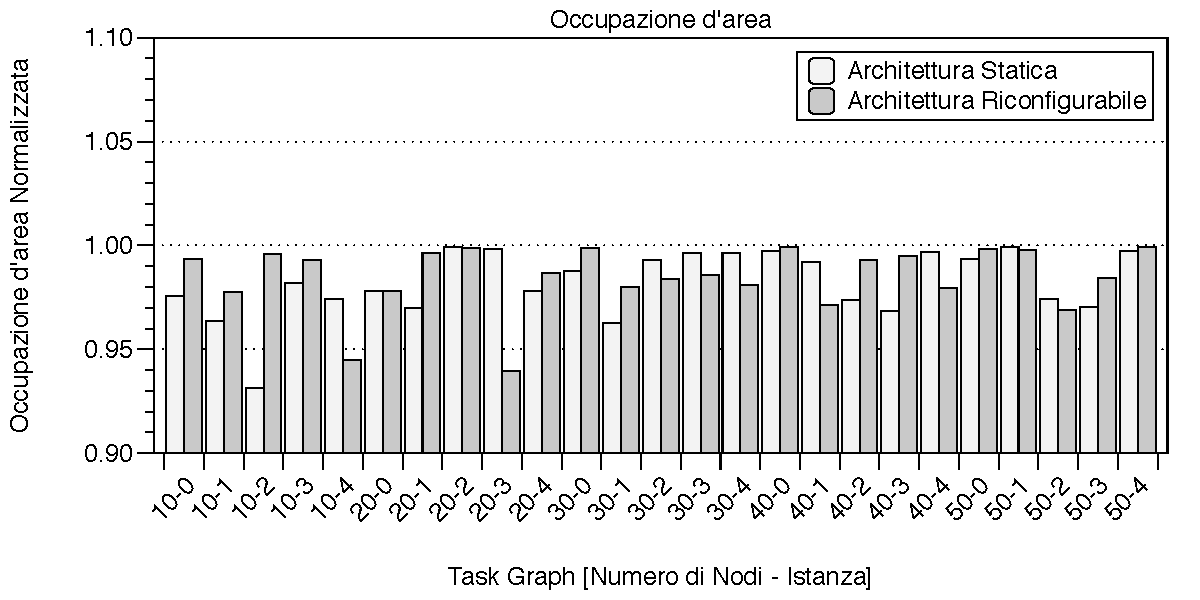
\includegraphics[width=\textwidth]{./capitoli/figure/cap6/FPL_Area.pdf}
  \caption{Uso dell'area, normalizzato rispetto all'area totale.}
  \label{fig:usoArea}
 \end{center}
\end{figure}


\begin{figure}[t]
 \begin{center}
  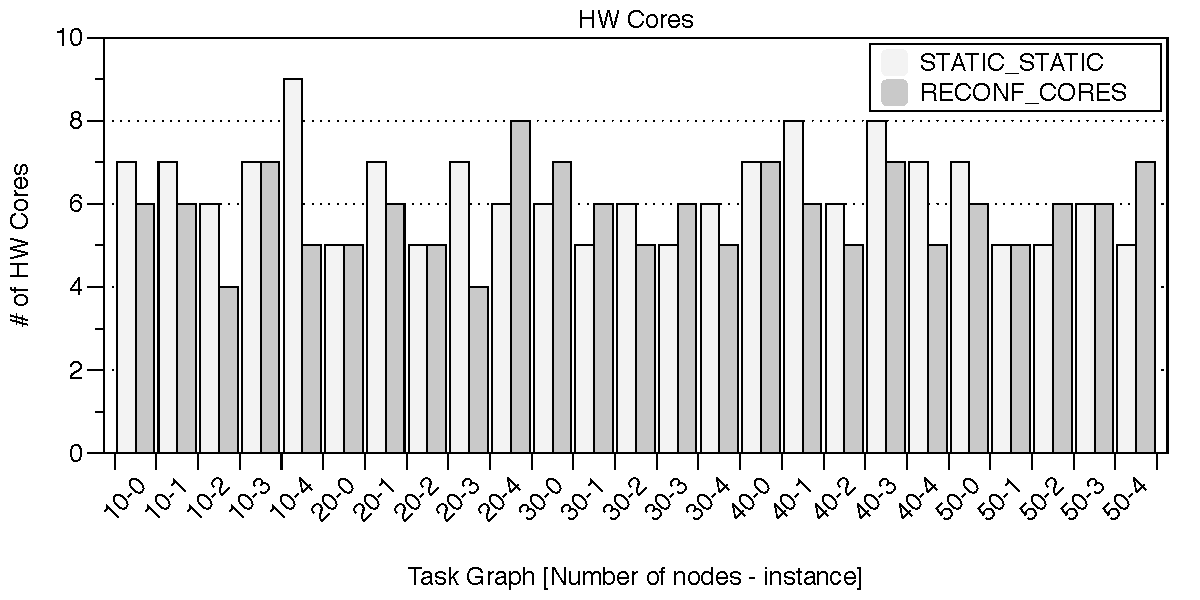
\includegraphics[width=\textwidth]{./capitoli/figure/cap6/FPL_HWcores.pdf}
  \caption{Numero di core utilizzati con architettura statica e riconfigurabile.}
  \label{fig:coreUtilizzati}
 \end{center}
\end{figure}


\begin{figure}[t]
 \begin{center}
  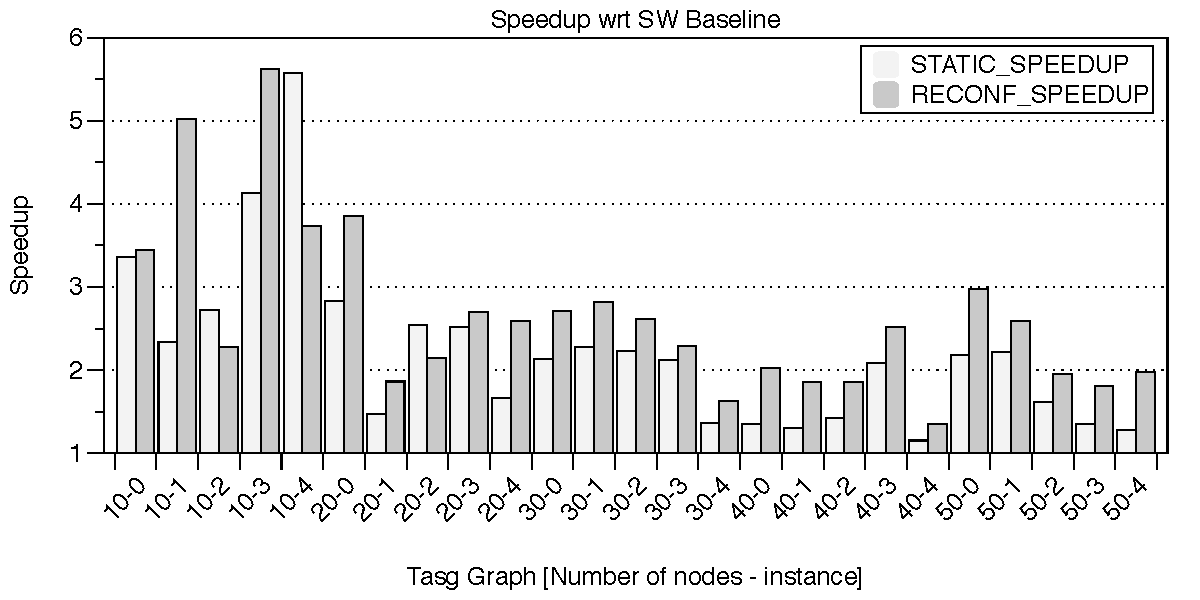
\includegraphics[width=\textwidth]{./capitoli/figure/cap6/FPL_makespan.pdf}
  \caption{Speedup dell'architettura statica e riconfigurabile rispetto alla
  baseline software.}
  \label{fig:speedupBaseline}
 \end{center}
\end{figure}


\begin{figure}[t]
 \begin{center}
  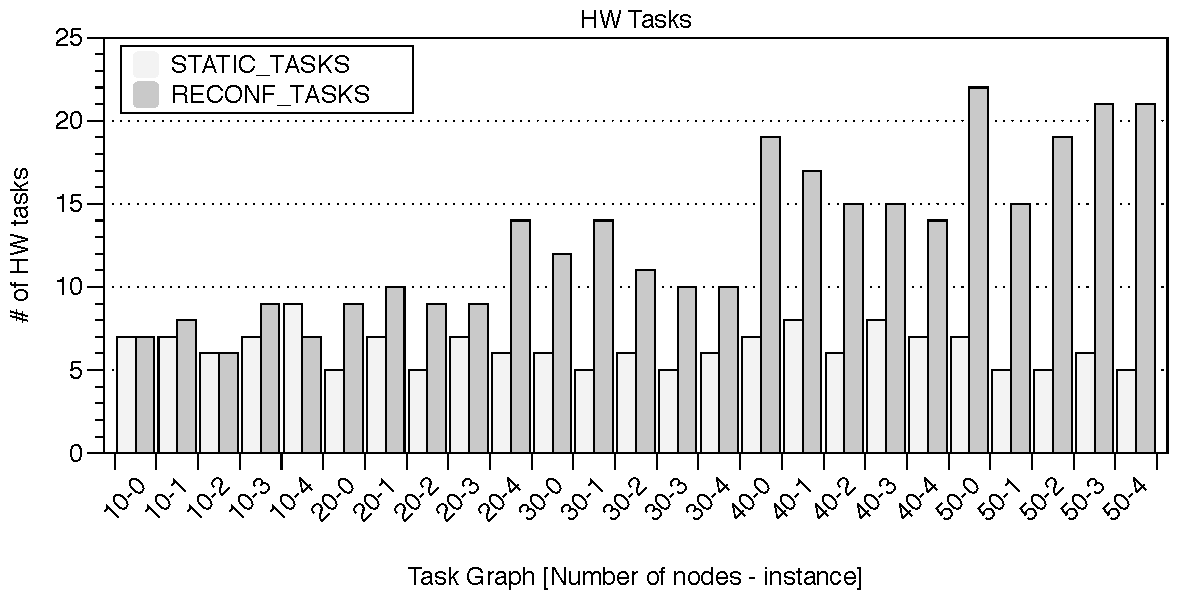
\includegraphics[width=\textwidth]{./capitoli/figure/cap6/FPL_HWtasks.pdf}
  \caption{Numero di task mappati su processing element statici e riconfigurabili.}
  \label{fig:hardwareTask}
 \end{center}
\end{figure}


\begin{figure}[t]
 \begin{center}
  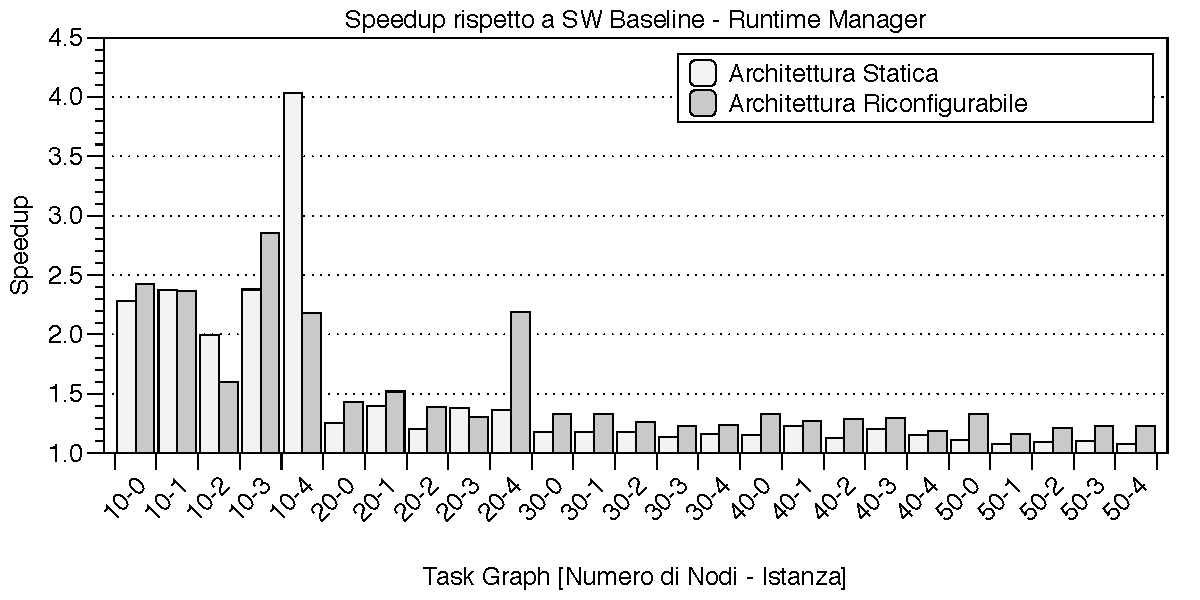
\includegraphics[width=\textwidth]{./capitoli/figure/cap6/FPL_Runtime.pdf}
  \caption{Speedup dell'architettura statica e riconfigurabile rispetto alla
  baseline software, dopo l'esecuzione sul dispositivo.}
  \label{fig:speedupBaselineRuntime}
 \end{center}
\end{figure}